\subsection{Addressing Parameterised circuit depth}
\subsubsection{Shallow Circuits, Local Cost Function}
\begin{figure} 
    \centerline{
        \Qcircuit @C=1em @R=0em {
        & \multigate{4}{U(\theta)}    & \meter\\
        & \ghost{U(\theta)}           & \meter\\
        & \ghost{U(\theta)}           & \meter\\
        & \ghost{U(\theta)}           & \meter\\
        & \ghost{U(\theta)}           & \meter\\
        }
    }
    \centerline{a) Global Cost Function}
    \centerline{
        \Qcircuit @C=1em @R=0em {
        & \multigate{4}{U(\theta)}    & \meter\\
        & \ghost{U(\theta)}           & \qw\\
        & \ghost{U(\theta)}           & \qw\\
        & \ghost{U(\theta)}           & \qw\\
        & \ghost{U(\theta)}           & \qw\\
        }
    }
    \centerline{b) Local Cost Function}
    \caption{
        An illustrative example of Global Cost Function and Local Cost Function.
        a) Global Cost Function compares the states in exponentially large Hilbert space.
        b) Local Cost Function compares the states at the qubit level.
    }\label{cost functions}
\end{figure}

Cerezo et al. has demonstrated \cite{cerezoCostFunctionDependent2021} the properties of a 'local cost function' in a parameterised circuit. 
Let us recall the cost function $C$ with an operator $O$, the ansatz $U(\theta)$ and some input states $\rho$:
\begin{equation}
    C = \Tr\left[
    OU(\theta) \rho U^\dagger(\theta)
    \right],
\end{equation}
the authors called this cost function as 'Global Cost Function' $C_G$, which can inhabit Barren Plateaus. Compared to the proposed 'Local Cost Function':
\begin{equation}
    C_L = \Tr\left[
    O_L U(\theta) \rho U^\dagger(\theta)
    \right],
\end{equation}
with
\begin{equation}
    O_L = I- \frac{1}{n} \sum^n_{j=1}\rho_j \bigotimes I_{\overline{j}},
\end{equation}
where $I_{\overline{j}}$ is the identity on all qubits except the qubit in $j$-th position.

\begin{figure}
    \centering
    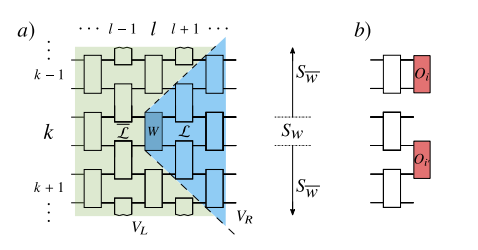
\includegraphics[scale=0.5]{LiteratureReview/Appendices/alterlayeransatz.png}
    \caption{
        Altering Layered Ansatz. 
        a) Each parameterized block $W_{kl}$ acts on $m$ qubits.
        $S_k$ is the $m$ qubit subsystem on which $W_{kL}$ acts, note that L is the last layer of the ansatz $U(\theta)$.
        The right (or forward) light-cone $\mathcal{L}$ contains all the gates with at least one input to $W$, $\overline{\mathcal{L}}$ is the opposite.
        $S_w$ is the subsystem of $m$ qubits which $W$ acts on, and $S_{\overline{w}}$ is the subsystem of $m$ qubits which $W$ have limited connection.
        b) The example of operator $O_i$ acts non-trivially in the subsystem $S_{k-1}$ only, while the operator $O_{i'}$ acts non-trivially on the second half ($m/2$) qubits of $S_k$ and on the first half ($m/2$) qubits of $S_{k+1}$.
        Figure from Ref \cite{cerezoCostFunctionDependent2021}
    }
    \label{Altering Layered Ansatz}
\end{figure}

The authors introduced the Altering Layered Ansatz $U(\theta)$ with $L$ layers of $m$-qubit unitaries $W_{kl}(\theta_{kl})$ (see Figure \ref{Altering Layered Ansatz}).
If a local cost function is used for this Altering Layered Ansatz, then there is a lower bound for the variants of the gradients that depends on the number of qubits and some configurations of the circuit. 
For a $L$-layered ansatz, let the variance $\mathrm{Var}[\partial_v C]$ of the partial derivative of the cost function $C$, the lower bound $G_n$ for the variance is:
\begin{equation}
    G_n(L,l) \leq \mathrm{Var}[\partial_k C]
\end{equation}
\begin{equation}
    G_n(L,l) = \frac{{2}^{m(l+1)-1}}{{({2}^{2m}-1)}^{2}{({2}^{m}+1)}^{L+l}}
    \times \mathop{\sum}\limits_{i\in {i}_{{\mathcal{L}}}}\mathop{\sum}\limits _{{(k,k^{\prime} )\in {k}_{{{\mathcal{L}}}_{\text{B}}}}\atop {k^{\prime} \geqslant k}}{c}_{i}^{2}\epsilon ({\rho }_{k,k^{\prime} })\epsilon ({\widehat{O}}_{i})\ ,
\end{equation}
Where the forward light-cone $\mathcal{L}$ is a set of gates with at least one input connected to the output of a block $W$; 
$S_k$ is the $m$-qubit subsystem;
$i_{\mathcal{L}}$ is a set of indices such that the operators $\hat{O_i}$ act on qubits in $\mathcal{L}$;
$k_{\mathcal{L}_B}$ is a set of indices such that the subsystem $S_k$ in the backward light-cone $\mathcal{L}_\text{B}$ of block $W$ (see Figure \ref{Forward-backward light cone} for example).
\begin{figure}
    \centering
    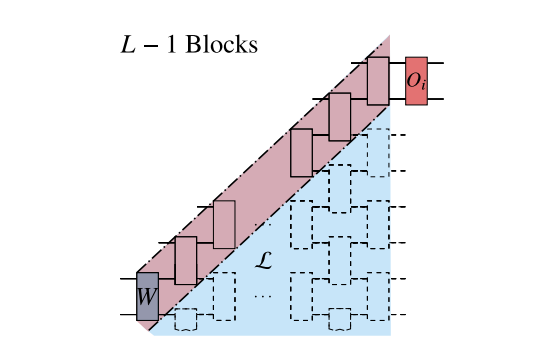
\includegraphics[scale=0.5]{LiteratureReview/Appendices/lightcone.png}
    \caption{
        An illustrative example of backward and forward light-cone.
        The operator $O_i$ in the topmost is in the scope of the forward light-cone $\mathcal{L}$ of block $W$.
        The thick-line dashes indicate the backward light-cone $\mathcal{L}_{\text{B}}$ of the operator $O_i$.
        Figure from Ref \cite{cerezoCostFunctionDependent2021}
    }
    \label{Forward-backward light cone}
\end{figure}

If the total depth $L$ is in the range $O(\log(n))$ of the number of qubits (a shallow configuration), then the lower bound cannot vanish faster than $\Omega(1/\mathrm{poly}(n))$. 
Thus, no Barren Plateau occurs in this case.



\subsubsection{Layerwise learning for quantum neural networks}

There is another method that manipulates the circuit depth throughout the training period studied by Skolik et al. \cite{skolikLayerwiseLearningQuantum2021}. 
In more detail, the algorithm consists of two phases:

\textbf{The first phase} constructs the ansatz by adding layers one by one, with the parameters are all initially zero. For a small number $s$ of starting layers, the set of parameters $\vec{\theta_1}$, and $W$ operators connecting qubits, then the initial layers $l_1(\vec{\theta_1})$ is presented:

\begin{equation}
    l_1(\vec{\theta_1})
    = \prod_{j=1}^s U_{1_j}(\vec{\theta_{1_j}}) W \;,
\end{equation}

Where each consecutive layer $l_i(\vec{\theta_i})$ of form
\begin{equation}
    l_i(\vec{\theta_i})
    =U_i(\vec{\theta_i}) W \;,
\end{equation}
is added after a certain number of epochs and the previous layers' parameters become fixed. 
One epoch is the set of iterations for the algorithm to see each training sample; an update of all trainable parameters is called one iteration.

This process can stop when a certain circuit depth is reached or until the objective function's value does not improve with additional layers.
Figure \ref{ll circuit} provides an illustrative example of the final circuit.
Eventually, we obtain the final circuit of $L$ layers:

\begin{equation}
    U(\vec{\theta})
    = \prod_{i=0}^L l_i (\vec{\theta_i}) \;.
\end{equation}
\begin{figure} 
    \centerline{
        \Qcircuit @C=1em @R=0em {
        & \multigate{4}{l_1(\vec{\theta_1})}    & \multigate{4}{l_2(\vec{\theta_2})}    & \qw &        & & \multigate{4}{l_i(\vec{\theta_i})}   & \qw\\
        & \ghost{l_1(\vec{\theta_1})}           & \ghost{l_2(\vec{\theta_2})}           & \qw &        & & \ghost{l_i(\vec{\theta_i})}          & \qw\\
        & \ghost{l_1(\vec{\theta_1})}           & \ghost{l_2(\vec{\theta_2})}           & \qw & \cdots & & \ghost{l_i(\vec{\theta_i})}          & \qw\\
        & \ghost{l_1(\vec{\theta_1})}           & \ghost{l_2(\vec{\theta_2})}           & \qw &        & & \ghost{l_i(\vec{\theta_i})}          & \qw\\
        & \ghost{l_1(\vec{\theta_1})}           & \ghost{l_2(\vec{\theta_2})}           & \qw &        & & \ghost{l_i(\vec{\theta_i})}          & \qw\\
        }
    }
    \caption{
        Constructing the ansatz from shallow layers.
    }\label{ll circuit}
\end{figure}


\textbf{The second phase} takes the pre-trained circuit from phase one and trains \almarginpar{What are these?}\underline{larger adjacent partitions} of layers at a time.
In more detail, we can set a parameter $r$ to specify the percentage of parameters to be trained in one step, e.g. one third, or a quarter of the circuit layers.